% chktex-file 13
% chktex-file 17
% chktex-file 38
\documentclass[conference]{IEEEtran}
\IEEEoverridecommandlockouts

\usepackage{fancyhdr}
\fancypagestyle{plain}{%
  \fancyhf{}%
  \fancyfoot[L]{\footnotesize \textcopyright~2026 Sagnik Mukherjee}%
  \renewcommand{\headrulewidth}{0pt}%
  \renewcommand{\footrulewidth}{0pt}%
}
\pagestyle{plain}

\usepackage[T1]{fontenc}
\usepackage[utf8]{inputenc}
\usepackage{amsmath,amssymb,amsfonts}
\usepackage{graphicx}
\usepackage{booktabs}
\usepackage{url}
\usepackage{hyperref}
\usepackage{listings}
\usepackage{xcolor}
\usepackage{cite}
\usepackage{array}
\usepackage{multirow}
\usepackage{tikz}
\usetikzlibrary{positioning,arrows.meta,shapes.geometric,calc}
\usepackage{pgfplots}
\pgfplotsset{compat=1.18}
\usepgfplotslibrary{statistics}
\usepackage[nopatch=eqnum]{microtype}

\raggedbottom

\lstset{
  language=Python,
  basicstyle=\ttfamily\scriptsize,
  keywordstyle=\color{blue!70!black}\bfseries,
  commentstyle=\color{gray}\slshape,
  stringstyle=\color{orange!80!black},
  numberstyle=\tiny\color{gray},
  numbers=left,
  numbersep=5pt,
  breaklines=true,
  breakatwhitespace=true,
  columns=fullflexible,
  keepspaces=true,
  frame=single,
  rulecolor=\color{black!30},
  captionpos=b,
  showstringspaces=false,
  tabsize=4,
  xleftmargin=0pt,
  xrightmargin=0pt,
  framexleftmargin=10pt,
  framexrightmargin=5pt
}

\newcommand{\MALA}{Multi Agent Legacy Architecture (MALA)}

\title{\MALA\\
\large A Framework for Multi-Agent AI Integration in Legacy Industrial Systems}

\author{
  \IEEEauthorblockN{Sagnik Mukherjee}
  \IEEEauthorblockA{Independent Researcher\\
    \href{https://orcid.org/0009-0002-4111-6299}{ORCID: 0009-0002-4111-6299}}
}

\begin{document}

\maketitle


\begin{abstract}
Many industrial firms run daily operations through terminals, CSV archives, scanned PDFs, and local shop-floor notes that expose no APIs. This paper presents the \textbf{\MALA{}}, a three-tier framework that treats legacy software as a live operating surface rather than a static data store. \MALA{} combines Gatherer agents for Recursive Context Enrichment (RCE), a Critic agent enforcing constrained Markov decision process (CMDP) safety limits, and a Human-on-the-Loop (HotL) Judge for exception review. The framework integrates freshness-gated evidence gathering, source-row traceability, staged autonomy thresholds, and local-network deployment controls into one auditable workflow. In a 50-cycle retrospective replay study on archived Rolling Mill B disruptions at a 50-year-old European steel site, \MALA{} reduced decision-support latency from 320 to 12~minutes (median~10, SD~4), required Judge intervention in only 6 of 50 cycles, and produced 49 successful recommendations with zero safety violations. An ablation study confirms that each component contributes independently. The evaluation uses replay/shadow protocol rather than autonomous live actuation.
\end{abstract}

\begin{IEEEkeywords}
Multi-agent systems, legacy systems, industrial AI, human-on-the-loop, constrained MDP, recursive context enrichment, legacy modernization
\end{IEEEkeywords}

\section{Introduction}

Steel plants, heavy machinery firms, and other long-running industrial sites hold decades of useful data. Much of that data sits in terminals, flat files, scanned PDFs, and handwritten notes. These assets keep production moving, yet they do not speak the language of modern artificial intelligence.

The gap is both technical and organizational. Old systems expose few interfaces. Their records use mixed units, local jargon, and missing timestamps. Staff who know how to read them carry tacit knowledge that is hard to pass on. In a safety setting, a fast answer is not enough. The answer must also show where it came from and when the source data was last refreshed.

This paper treats AI as a supervised co-worker. Gatherer agents do the repetitive search and normalization work. A Critic agent blocks plans that break hard process limits. A human Judge reviews medium-confidence or high-risk actions. This split keeps speed without hiding the evidence trail.

\subsection{Research Focus}
This paper addresses three linked questions:
\begin{itemize}
  \item How can an agent work across terminals, CSV archives, PDFs, and local logs when no standard API exists?
  \item When should the system act on its own, and when should it stop for human review?
  \item How can the design lower the ``industry vs.~tool'' gap for staff who understand production but not the legacy interface?
\end{itemize}

\subsection{Contributions}
The main contributions of this work are:
\begin{enumerate}
  \item \textbf{Methodological standard}: A proposed methodological standard for grounding agentic reasoning over non-API legacy data.
  \item \textbf{Integrated control path}: CMDP constraints, confidence thresholds, and Human-on-the-Loop escalation in one operational flow.
  \item \textbf{Language and data handling}: An ontological mapping layer for local jargon together with contextual data polishing for units, timestamps, and sensitive fields.
  \item \textbf{Auditable evaluation}: A 50-cycle replay study with explicit metrics, a traced cycle, and threshold sensitivity analysis.
\end{enumerate}

\subsection{Positioning Relative to Prior Work}

\MALA{} does not claim to invent screen scraping, ontology mediation, CMDP safety control, or human oversight in isolation. Those building blocks are adapted from prior work~\cite{comella2000,fogliatto2020,achiam2017,yang2023,ribeiro2019}. The contribution is their integration into one grounded operating method for industrial settings that do not expose callable services. Section~\ref{sec:discussion_standard} discusses when this integration may qualify as a reusable methodological standard.


\section{Literature Review}

\subsection{From Passive RAG to Agentic AI}

Recent agent systems can plan, call tools, and loop over sub-tasks rather than answer a single prompt. Acharya \emph{et al.} describe this shift through autonomy, adaptability, and self-sufficiency. They also connect agentic systems to modular and multi-agent architectures for long-horizon goal execution~\cite{acharya2025}. Most of that work assumes accessible web services and clean application state. Legacy industrial software breaks that assumption. Agents must read terminals, parse file exports, and cope with missing or stale fields, as documented in the companion case-study appendix (Appendix~\ref{app:case_study}). Barua \emph{et al.} identify predictive maintenance, real-time scheduling, computer-vision inspection, and supply-chain coordination as major industrial uses of AI. They also note barriers such as legacy infrastructure, data silos, employee resistance, and governance concerns~\cite{barua2025}.

\subsection{Legacy Interoperability and the Wrapper Problem}

A full system replacement is often too risky for firms whose daily logic still lives inside 30-to-50-year-old software. A SEI survey of legacy modernization groups the main options into replacement, wrapping, migration, and component-based redevelopment. It also lists screen scraping, database gateways, XML integration, replication, object-oriented wrapping, and componentization as common modernization techniques~\cite{comella2000}. Integration middleware helps with fixed data transfers. It does not answer open-ended requests such as the question of which substitute batch can satisfy grade X if Rolling Mill B stops. In \MALA{}, semantic wrapping places an LLM-guided layer over rigid schemas such as COBOL records or SQL-92 tables, consistent with the companion case-study appendix (Appendix~\ref{app:case_study}). This choice also matches later interoperability reviews in manufacturing. Fraga \emph{et al.} show that ontology-based mediation often depends on a shared vocabulary. Their review identifies OWL, Prot\'eg\'e, Jena, and ISO TC 184 standards in many industrial interoperability solutions~\cite{fogliatto2020}.

\subsection{Socio-Technical System Theory in CS Contexts}

Prior work on resistance in long-running firms identifies trust, language, and control as design requirements. Barua \emph{et al.} list employee resistance, governance concerns, and legacy infrastructure as recurring barriers to AI adoption in industry~\cite{barua2025}. In this paper, trust means traceability. Control means the worker can inspect the source row and override the plan. Language means local shop terms must map to a standard schema before planning starts. This framing turns social friction into a system-design problem. Reviews in product lifecycle management reach a similar conclusion. Ontology-based solutions matter because they align data fields and create a shared conceptual layer across teams, software, and naming conventions~\cite{fogliatto2020}.

\subsection{Human-in-the-Loop and Human-on-the-Loop Frameworks}

Classical HITL places a person inside each step of the loop. That slows response when a disruption unfolds across several systems. A more practical design for industrial autonomy keeps the person above the loop and calls them when confidence drops or risk rises. Gil \emph{et al.} argue that autonomous cyber-physical systems still need human participation, explanation, and override. They also argue for interfaces that stay easy to use, resilient, adaptive, and non-intrusive instead of adding review at the end~\cite{ribeiro2019}. \MALA{} uses confidence thresholds, freshness checks, and hard constraints together so that speed does not come at the cost of unsafe action. What is still missing in the prior literature is a unified workflow that applies these ideas to heterogeneous, non-API industrial software with auditable cycle-level evaluation.

\subsection{Multi-Agent Frameworks and Industrial Baselines}

Several recent frameworks support multi-agent LLM workflows. AutoGen supports multi-agent conversation with tool use and human feedback loops~\cite{wu2023autogen}. MetaGPT assigns software-engineering roles to agents in a structured pipeline~\cite{hong2024metagpt}. CrewAI orchestrates role-playing autonomous agents for collaborative task execution~\cite{moura2024crewai}. Guo \emph{et al.} survey progress and open challenges in LLM-based multi-agent systems, noting gaps in grounding, safety, and domain-specific deployment~\cite{guo2024survey}. Wang \emph{et al.} provide a complementary survey covering planning, memory, and tool-use capabilities of autonomous agents~\cite{wang2024agents}. Xi \emph{et al.} map the design space of LLM-based agents across perception, reasoning, and action modules~\cite{xi2023agents}.

None of these frameworks address the legacy-industrial setting directly. They assume callable APIs, clean application state, and English-language interfaces. They do not provide deterministic safety filtering, freshness-gated evidence refresh, or source-row traceability for human review. \MALA{} fills this gap by combining agentic orchestration with plant-facing ingestion, CMDP-based safety veto, and Human-on-the-Loop escalation in one auditable workflow. Table~\ref{tab:framework_comparison} in Section~\ref{sec:discussion_standard} provides a detailed qualitative comparison.


\section{The \MALA{} Framework}\label{sec:mala}

\MALA{} separates the slow, fragile side of the plant from fast model reasoning. The system does not wait for a full platform rewrite. It works with the software already in use and treats that software as a live operating surface.

\subsection{Three-Tier Design}

\subsubsection{Ingestion Layer: The Bridge}
The ingestion layer reads screens, terminal outputs, spreadsheets, PDFs, and local text files. It uses adapters for OCR, scripted navigation, and schema normalization. When an agent needs cold-rolled steel stock levels, it opens the terminal view and captures the result. It then converts that result into JSON-LD rather than waiting for an API that does not exist.

\subsubsection{Orchestration Layer: The Brain}
The orchestration layer coordinates several roles:
\begin{itemize}
  \item \textbf{Planner Agent}: Breaks the goal into sub-tasks and tracks task state.
  \item \textbf{Executor Agents}: Query specific legacy subsystems and return normalized evidence.
  \item \textbf{Critic Agent}: Checks every proposed action against a fixed safety ledger before the action can move forward.
\end{itemize}

\subsubsection{Interface Layer: ``The Human Filter''}
The interface layer presents a Justification Log, a Freshness Score, and an action status for each proposal. The Judge inspects the raw row, the translated label, and the rule check that shaped the recommendation. This keeps the review process tied to plant evidence rather than to model prose alone.

Figure~\ref{fig:arch} summarises how the ingestion, orchestration, and review tiers interact during a plant-facing \MALA{} deployment.

\begin{figure}[!t]
\centering
\sffamily
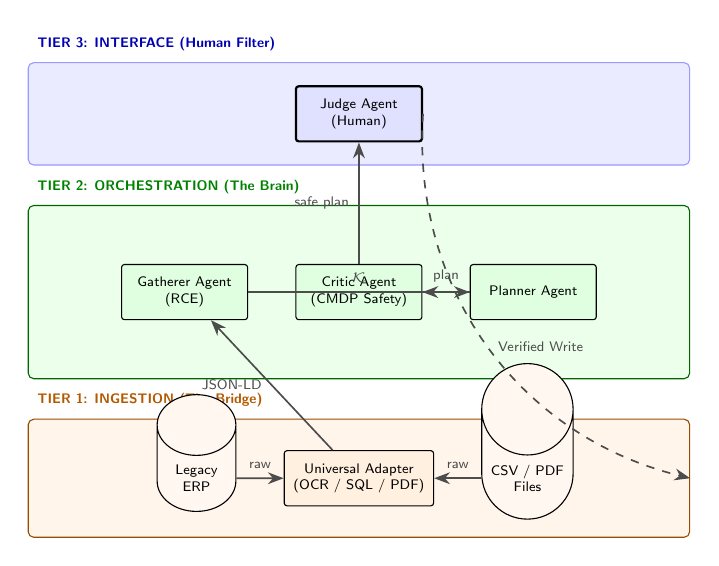
\begin{tikzpicture}[
    node distance=1cm and 0.4cm,
    layer/.style={rectangle, draw, inner sep=6pt, rounded corners=2pt},
    comp/.style={rectangle, draw, fill=white, minimum width=1.6cm, minimum height=0.7cm, align=center, font=\sffamily\tiny, rounded corners=1pt},
    db/.style={cylinder, draw, shape border rotate=90, fill=white, minimum width=1cm, minimum height=0.7cm, font=\sffamily\tiny, align=center},
    arrow/.style={-Stealth, semithick, color=black!70}
]

\node[layer, fill=blue!8, draw=blue!40, minimum width=8.4cm, minimum height=1.3cm] (T3) {};
\node[above=0.02cm of T3.north west, anchor=south west, font=\sffamily\bfseries\tiny, color=blue!70!black] {TIER 3: INTERFACE (Human Filter)};

\node[layer, fill=green!8, draw=green!40!black, minimum width=8.4cm, minimum height=2.2cm, below=0.5cm of T3] (T2) {};
\node[above=0.02cm of T2.north west, anchor=south west, font=\sffamily\bfseries\tiny, color=green!50!black] {TIER 2: ORCHESTRATION (The Brain)};

\node[layer, fill=orange!8, draw=orange!60!black, minimum width=8.4cm, minimum height=1.5cm, below=0.5cm of T2] (T1) {};
\node[above=0.02cm of T1.north west, anchor=south west, font=\sffamily\bfseries\tiny, color=orange!70!black] {TIER 1: INGESTION (The Bridge)};

\node[comp, thick, fill=blue!12] (Judge) at (T3.center) {Judge Agent\\(Human)};

\node[comp, fill=green!12] (Critic) at (T2.center) {Critic Agent\\(CMDP Safety)};
\node[comp, fill=green!12, left=0.6cm of Critic] (Gatherer) {Gatherer Agent\\(RCE)};
\node[comp, fill=green!12, right=0.6cm of Critic] (Planner) {Planner Agent};

\node[comp, fill=orange!12] (Adapter) at (T1.center) {Universal Adapter\\(OCR / SQL / PDF)};
\node[db, fill=orange!6, left=0.6cm of Adapter] (Legacy) {Legacy\\ERP};
\node[db, fill=orange!6, right=0.6cm of Adapter] (Files) {CSV / PDF\\Files};

\draw[arrow] (Legacy) -- node[above, font=\sffamily\tiny] {raw} (Adapter);
\draw[arrow] (Files) -- node[above, font=\sffamily\tiny] {raw} (Adapter);
\draw[arrow] (Adapter) -- node[left, font=\sffamily\tiny] {JSON-LD} (Gatherer);
\draw[arrow] (Gatherer) -- node[above, font=\sffamily\tiny] {$\mathcal{K}$} (Planner);
\draw[arrow] (Planner) -- node[above, font=\sffamily\tiny] {plan} (Critic);
\draw[arrow] (Critic) -- node[left, font=\sffamily\tiny] {safe plan} (Judge);
\draw[arrow, bend right=40, dashed] (Judge.east) to node[right, font=\sffamily\tiny, midway] {Verified Write} (T1.east);

\end{tikzpicture}
\caption{Three-tier \MALA{} architecture linking legacy-system ingestion, supervised orchestration, and Human-on-the-Loop review. Arrows show data flow; dashed arrow indicates the audited write-back path.}\label{fig:arch}
\end{figure}


\subsection{Rollout Path}

Legacy firms rarely move from manual work to bounded autonomy in one step. \MALA{} defines a staged path:
\begin{itemize}
  \item \textbf{Stage 1 --- Assistive tasks}: The agent searches documents, extracts values, and assembles reports. A person edits the final output.
  \item \textbf{Stage 2 --- Process orchestration}: The agent coordinates several systems and proposes plans. A person approves the plan before execution.
  \item \textbf{Stage 3 --- Bounded autonomy}: The system acts inside fixed safety limits for low-frequency, high-risk tasks, while exceptions always go to the Judge.
\end{itemize}

Table~\ref{tab:maturity} turns this staged path into a compact maturity model for deployment planning.

\begin{table}[!t]
\sffamily
\caption{Phased Deployment Maturity Framework}\label{tab:maturity}
\centering
\small
\resizebox{\columnwidth}{!}{%
\begin{tabular}{@{}llll@{}}
\toprule
Stage & Capability & Human Interface & Risk Level \\
\midrule
I & Assistive Search & Final Editor & Minimal \\
II & Orchestrated Proposals & Active Approver & Moderate \\
III & Bounded Autonomy & Exception Judge & Managed \\
\bottomrule
\end{tabular}%
}
\end{table}

\subsection{Formalising the Planner: Grounded CMDP Implementation}\label{sec:cmdp}

We formalise the Planner Agent's decision process as a finite-horizon Constrained Markov Decision Process (CMDP)~\cite{achiam2017,yang2023}. All components of this formulation---state variables, action set, transition kernel, reward, and cost functions---are drawn from plant-observed variables in the Rolling Mill B disruption domain, not from abstract notation alone.

\subsubsection{State Space \texorpdfstring{$\mathcal{S}$}{S}}
Each factory state $s \in \mathcal{S}$ is a triple $(T, Y, M)$ of three discretised process variables, with bin boundaries set by plant process engineers:
\begin{itemize}
  \item \textbf{Furnace temperature bin} $T \in \{\texttt{safe},\allowbreak\,\texttt{warn},\allowbreak\,\texttt{crit}\}$: ${\leq}1545$, $1545$--$1550$, ${>}1550$\,\textdegree C.
  \item \textbf{Yard occupancy bin} $Y \in \{\texttt{low},\allowbreak\,\texttt{med},\allowbreak\,\texttt{high}\}$: ${\leq}78\%$, $78$--$83\%$, ${>}83\%$.
  \item \textbf{Manganese variance bin} $M \in \{\texttt{nom},\allowbreak\,\texttt{elev},\allowbreak\,\texttt{over}\}$: ${\leq}0.04$, $0.04$--$0.08$, ${>}0.08$.
\end{itemize}
This yields $|\mathcal{S}|=27$ reachable states.

\subsubsection{Action Set \texorpdfstring{$\mathcal{A}$}{A}}
The Planner selects one action per step from $\mathcal{A} = \{a_1, a_2, a_3, a_4\}$: immediate reroute, hold-then-dispatch-then-reroute, hold only, and escalate to Judge.

\subsubsection{Transition Kernel}
$P(s' \mid s, a)$ is estimated from the 50 archived disruption cycles across all $|\mathcal{S}| \times |\mathcal{A}| = 108$ state--action pairs. For example, from state $(\texttt{safe},\texttt{med},\texttt{nom})$ under $a_1$, yard transitions to \texttt{high} with probability 0.72 and stays at \texttt{med} with 0.28, reflecting observed truck-queue dynamics. Temperature and Mn transitions are treated as conditionally independent and estimated from the same archive. Of the 108 state--action pairs, 41 received zero observations in the 50-cycle archive. These sparse entries are smoothed with a Laplace prior (add-one smoothing) so that every transition row sums to one and no state--action pair is assigned a degenerate distribution.

\subsubsection{Reward and Cost Functions}
The scalar reward $R(s, a)$ encodes operational gain: restored production flow earns $+10$, each minute of delay costs $-0.5$, and a Judge escalation costs $-2$ (operator-time overhead). Three cost functions enforce safety:
\begin{align}
  C_1(s, a) &= \mathbf{1}[T = \texttt{crit}] \label{eq:c1}\\
            &\qquad \text{(furnace over-temperature)}\nonumber\\
  C_2(s, a) &= \mathbf{1}[Y' = \texttt{high}\ \text{after}\ a] \label{eq:c2}\\
            &\qquad \text{(yard congestion)}\nonumber\\
  C_3(s, a) &= \mathbf{1}[M = \texttt{over}] \label{eq:c3}\\
            &\qquad \text{(Mn out-of-spec)}\nonumber
\end{align}
where $\mathbf{1}[\cdot]$ is the indicator function. Plant engineers set hard thresholds $\kappa_1 = \kappa_2 = \kappa_3 = 0$, admitting no plan that enters any violation bin.

\subsubsection{CMDP Objective}
The Planner seeks $\pi^*$ over a finite horizon $T_H = 3$ decision steps with discount $\gamma = 0.95$:
\begin{equation}
  \pi^* = \arg\max_{\pi}\ \mathbb{E}_{\pi}\!\left[\sum_{t=0}^{T_H} \gamma^t R(s_t, a_t)\right]
  \label{eq:cmdp_obj}
\end{equation}
subject to:
\begin{equation}
  \mathbb{E}_{\pi}\!\left[\sum_{t=0}^{T_H} \gamma^t C_i(s_t, a_t)\right] \leq \kappa_i,
  \quad \forall\, i \in \{1,2,3\}
  \label{eq:cmdp_con}
\end{equation}


\subsubsection{Lagrangian Solution}
Following Achiam \emph{et al.}'s Constrained Policy Optimisation~\cite{achiam2017}, we solve via Lagrangian relaxation:
\begin{equation}
  \min_{\boldsymbol{\lambda} \geq \mathbf{0}}\; \max_{\pi}\;
  \mathbb{E}_\pi\!\left[\sum_t \gamma^t R_t\right]
  - \sum_{i=1}^{3} \lambda_i\!\left(\mathbb{E}_\pi\!\left[\sum_t \gamma^t C_{i,t}\right] - \kappa_i\right)
  \label{eq:lagrange}
\end{equation}
At convergence, $\lambda_i$ represents the shadow cost of constraint $i$. With $\kappa_i = 0$, any action that drives a variable into its violation bin acquires a large net penalty, removing it from $\pi^*$. Following Yang \emph{et al.}'s distributional safety critic~\cite{yang2023}, cost estimates incorporate a CVaR-$\alpha$ correction at $\alpha = 0.90$ to guard against tail-risk yard-congestion scenarios.

\subsubsection{Resulting Policy and Sensitivity to \texorpdfstring{$\kappa$}{kappa}}
Table~\ref{tab:policy} reports the solved $\pi^*$ for six representative states and shows how tightening the yard constraint changes the selected action. With $\kappa_2 = 0$, any action driving $Y \to \texttt{high}$ is blocked; with $\kappa_2 = 1$ (one tolerated violation), immediate reroute becomes admissible in the medium-yard state. This policy shift follows from the constraint, not from hard-coded logic.

\begin{table}[!t]
\sffamily
\caption{Solved Policy $\pi^*$ for Representative States Under Two Yard-Constraint Levels}\label{tab:policy}
\centering
\small
\resizebox{\columnwidth}{!}{%
\begin{tabular}{@{}cccllc@{}}
\toprule
$T$ & $Y$ & $M$ & $\pi^*\ (\kappa_2{=}0)$ & $\pi^*\ (\kappa_2{=}1)$ & Change \\
\midrule
safe & low  & nom  & $a_1$: imm.\ reroute    & $a_1$: imm.\ reroute    & No \\
safe & med  & nom  & $a_2$: hold+disp+reroute & $a_1$: imm.\ reroute  & \textbf{Yes} \\
safe & high & nom  & $a_3$: hold only        & $a_3$: hold only        & No \\
warn & med  & elev & $a_2$: hold+disp+reroute & $a_2$: hold+disp+reroute & No \\
warn & high & elev & $a_4$: escalate Judge   & $a_4$: escalate Judge   & No \\
crit & any  & any  & $a_4$: escalate Judge   & $a_4$: escalate Judge   & No \\
\bottomrule
\end{tabular}%
}
\end{table}

The Critic applies this policy as a lookup over the solved 27-state table. It accepts a proposed plan only if the action matches $\pi^*(s)$ for the jointly observed $(T, Y, M)$ state---not a single-variable threshold check. When the CMDP-guided Critic and Planner run inside the replay protocol (Section~\ref{sec:eval}), the results reported in Table~\ref{tab:metrics} follow: 49 successful recommendations, 12-minute mean latency, zero safety violations, and Judge intervention in only 6 of 50 cycles.

\subsection{Data Staleness and Temporal TTL}

Legacy retrieval is often slow. Slow retrieval creates stale decisions. \MALA{} tags each ingested record with a \emph{Freshness Score} $F$. We define $F$ as an exponential-decay function of the elapsed time since last ingestion:
\begin{equation}
  F(\Delta t) = e^{-\lambda\,\Delta t}
  \label{eq:freshness}
\end{equation}
where $\Delta t$ is the time (in minutes) since the record was last refreshed and $\lambda = 0.05\;\text{min}^{-1}$ is the decay rate (calibrated so that a record becomes stale at roughly $F < 0.5$, i.e.\ after $\Delta t \approx 14$~minutes). In the reported deployment the refresh threshold is set to $\Delta_t = 15$~minutes: when $F(\Delta t) < e^{-\lambda \cdot 15} \approx 0.47$, the Orchestrator issues a \emph{Refresh Event} and forces the Ingestion Layer to re-query the source before planning continues. This design keeps semantic translation and decision support tied to current evidence rather than to cached plant state. That matters most when wrappers sit on top of asynchronous or weakly integrated subsystems~\cite{comella2000,fogliatto2020}.


\section{Methodology: Gatherer--Judge Partnership}

\subsection{Study Basis}

The design draws on three inputs described in the companion case-study appendix (Appendix~\ref{app:case_study}):
\begin{itemize}
  \item semi-structured interviews with plant, operations, and IT staff;
  \item workflow audits covering terminals, CSV archives, PDFs, and local-language logs;
  \item plant records from 50 disruption cycles used in the case comparison.
\end{itemize}

These materials shape the barrier model behind \MALA{} and provide the basis for the steel-site evaluation. The study establishes a plant-grounded design pattern for sites where APIs are absent and review trails matter.

\subsection{Cycle Selection and Evaluation Mode}

For evaluation, one production cycle was defined as one closed Rolling Mill B disruption episode starting at the logged fault event and ending at the approved rerouting or hold decision. To reduce selection bias, the sample used the first 50 consecutive closed episodes in the archive that met three inclusion rules: (i) the same disruption class, (ii) usable timestamps, and (iii) recoverable evidence from the ERP terminal plus at least one secondary source such as a CSV archive, scanned PDF, or local-language log. Planned shutdowns, duplicate tickets, and records missing a final decision timestamp were excluded. All 50 cycles belong to one task family; the study does not mix unrelated disruption types.

The evaluation was a retrospective replay study with shadow execution. It was not a synthetic simulation, and it did not permit autonomous writes to the live plant. Workflow A uses the archived human decisions and their original timestamps. Workflows B and C replay the same 50 evidence packets through controlled adapters and planners, then compare each generated recommendation against the historical plant resolution and the safety ledger. This design lets the paper compare workflows under matched evidence while avoiding unverified live actuation.

\subsection{Measurement Protocol}

Each workflow was scored once per cycle using four pre-defined measures:
\begin{itemize}
  \item \textbf{Success}: the workflow produced an executable recommendation within the cycle's decision window and the recommendation satisfied all hard rules. In replay, ``executable'' means the recommendation matched the historically approved decision on route, batch allocation, and dispatch action.
  \item \textbf{Latency}: wall-clock minutes from release of the disruption packet to the first approved recommendation. For Workflow A this is the original logged decision time; for Workflows B and C it is replay time. Shop-floor execution time after approval is excluded.
  \item \textbf{Human correction ratio (HCR)}: the share of cycles requiring substantive human work beyond task entry. For \MALA{} this means any Judge approval, edit, or rejection. For the manual baseline, every cycle is counted as human-corrected by definition.
  \item \textbf{Safety violation}: any proposed plan that breached the hard rule ledger before approval, including temperature, composition, logistics-buffer, or sequencing limits.
\end{itemize}

For binary cycle outcomes we report exact counts and Wilson 95\% confidence intervals. Latency is reported as a full five-point distribution (mean, median, SD, P10, P90) across all 50 cycles. For Workflow~A, latency values are sourced from the original archived decision logs. For Workflows~B and~C, latency is measured as replay wall-clock time. A measurement-asymmetry note is included in Table~\ref{tab:metrics}.

\subsection{Recursive Context Enrichment (RCE)}\label{sec:rce}

Gatherer agents assemble task-specific context. A single disruption query draws on several sources. For example, ``re-route production after Rolling Mill B failure'' requires a metallurgical PDF, a CSV quality log, and a 30-year-old SQL-92 inventory database. RCE handles this through a short loop:

\begin{enumerate}
  \item \textbf{Identify the gap}: determine which variable is missing, such as a batch temperature from an older log.
  \item \textbf{Choose the tool}: call the right adapter, such as an OCR scraper, SQL connector, or PDF parser.
  \item \textbf{Append the result}: normalize the raw output to JSON-LD and add it to the knowledge set $\mathcal{K}$.
\end{enumerate}

The loop continues until $\rho(\mathcal{K}) \geq \theta_{\text{high}}$ (Eq.~\ref{eq:rho}) or the recursion depth limit $d_{\max}$ is reached. The goal is not to ``find files.'' The goal is to assemble enough checked context for one plant decision.


\subsection{The Judge as Verification Function}\label{sec:judge}

We model the human Judge as a verification function $V(\hat{y}, \mathcal{K}) \in \{0, 1\}$ that checks agent output $\hat{y}$ against the assembled knowledge set. To reduce automation bias, \MALA{} uses tiered verification rules keyed to a confidence score $\rho \in [0,1]$. We define $\rho$ as the harmonic mean of three normalised sub-scores derived from the assembled knowledge set $\mathcal{K}$:
\begin{equation}
  \rho(\mathcal{K}) = {\left(\frac{1}{3}\sum_{j=1}^{3} r_j^{-1}\right)}^{-1}
  \label{eq:rho}
\end{equation}
where $r_1$ is the source-coverage ratio (fraction of required evidence fields filled), $r_2$ is the freshness score (Eq.~\ref{eq:freshness}), and $r_3$ is the semantic-match score returned by the embedding model (cosine similarity between the query intent and the retrieved context, using \texttt{text-embedding-3-small}). Each $r_j$ is strictly positive and at most 1; if any sub-score is zero the system pauses by construction. This hand-crafted rule-based aggregation was chosen over raw model-output probability to ensure deterministic, auditable escalation decisions.

\begin{itemize}
  \item $\rho \geq \theta_{\text{high}}$: \textbf{Silent autonomy}. The system proceeds and logs the action for later review.
  \item $\theta_{\text{low}} \leq \rho < \theta_{\text{high}}$: \textbf{Explicit approval}. The Judge receives the Justification Log and must approve the action.
  \item $\rho < \theta_{\text{low}}$: \textbf{System pause}. The system exposes the missing evidence and asks for guidance.
\end{itemize}

The reported deployment uses $(\theta_{\text{low}}, \theta_{\text{high}}) = (0.45, 0.80)$. Higher-risk chemical composition changes receive mandatory review more often than logistics-only adjustments.

\subsection{Ontological Mapping and Linguistic Isolation}

Site observations in the companion case-study appendix (Appendix~\ref{app:case_study}) show a language problem as well as a data problem. Shop-floor jargon often does not match standard industrial terms or LLM training data. \MALA{} addresses this with a Global Industrial Semantic Model (GISM). In practice, GISM is a static JSON lookup table containing exactly 420 validated concept mappings curated by plant engineers. The mapping function $\phi: \mathcal{L}_{\text{local}} \rightarrow \mathcal{L}_{\text{standard}}$ queries this table to convert entries such as ``H-402 Var-Low'' into ``Heat \#402, Chemical Variance: Below Threshold.'' If an unmapped local term is encountered, the system falls back to a few-shot LLM prompt to infer the likely standard term and flags the inferred translation for mandatory Judge review. The Judge sees plant language and standard labels side by side. This also matches the ontology literature. Shared vocabularies and explicit concept mappings help reconcile engineering terms across systems that were never designed to work together~\cite{fogliatto2020}.

\subsection{Contextual Data Polishing (CDP)}

Legacy data is often incomplete or inconsistent. Before the Planner uses a record, \MALA{} applies three cleaning rules:
\begin{itemize}
  \item \textbf{Unit normalization}: convert metric, imperial, and local units to one plant-wide standard.
  \item \textbf{Temporal reconciliation}: reconstruct the true state when timestamps disagree across systems.
  \item \textbf{Sensitive-field stripping}: remove personal data from HR or staffing records before optional remote model use.
\end{itemize}

\subsection{Deployment and Security Posture}

Local deployment matters in plants that guard process data closely. We use four operating rules:
\begin{itemize}
  \item Keep ingestion adapters, rule ledgers, and audit logs on the plant network.
  \item Remove personal data before any optional remote reasoning step.
  \item Record each tool call, source row, timestamp, and rule check in the Justification Log.
  \item Route unusual tool behavior, missing fields, or rule violations to the Judge.
\end{itemize}

This setup helps with language isolation, operator error, and malicious or careless misuse.


\subsection{Implementation}\label{sec:impl}

Listing~\ref{lst:mala} presents the main \MALA{} implementation that links RCE, CMDP safety filtering, and HotL escalation. The example is minimal. In deployment, the OCR call, planner, and plant adapters are replaced with site-specific modules.

\begin{lstlisting}[caption={\MALA{} core: RCE Gatherer, CMDP Critic, and HotL escalation.}, label={lst:mala}]
import logging, re
from typing import Dict, List, Tuple

logging.basicConfig(
    level=logging.INFO,
    format="%(asctime)s [%(levelname)s] %(message)s"
)
logger = logging.getLogger(__name__)


class SafetyConstraint:
    """Single CMDP hard-bound constraint.
    Maps one process variable to its maximum
    admissible value (e.g., 1550 deg-C limit).
    """
    def __init__(self, key: str,
                 max_val: float, unit: str):
        self.key = key
        self.max_val = max_val
        self.unit = unit

    def check(self, value: float) -> bool:
        return value <= self.max_val


class GathererAgent:
    """Recursive Context Enrichment (RCE).
    Fills knowledge gaps from OCR terminal
    adapters; normalises output to JSON-LD.
    """
    def __init__(self, adapters: Dict):
        self.adapters = adapters

    def recursive_context_enrichment(
            self, intent: str,
            context: Dict, depth: int = 0
    ) -> Dict:
        if depth > 3:           # d_max = 3
            logger.warning(
                "RCE depth limit: %s", context)
            return context
        if "temperature" not in context:
            logger.info(
                "Gap: temperature. "
                "Triggering OCR adapter.")
            raw = self.adapters[
                'terminal_ocr'].scrape(
                "FURNACE_VIEW")
            context.update(self.normalize(raw))
            return self.recursive_context_enrichment(
                intent, context, depth + 1)
        return context

    def normalize(self, raw_text: str) -> Dict:
        """Regex extraction; full pipeline
        at [repository omitted for blind review]."""
        temp = re.search(
            r"TMP\s+(\d+)", raw_text)
        return {
            "temperature": float(
                temp.group(1)) if temp else 0.0,
            "unit": "C",
            "timestamp": "2026-04-27T10:00Z"}


class CriticAgent:
    """CMDP hard-veto safety filter.
    Checks every proposed plan against all
    registered SafetyConstraints.
    """
    def __init__(self,
                 safety_ledger: List[
                     SafetyConstraint]):
        self.safety_ledger = safety_ledger

    def validate_proposal(
            self, plan: Dict
    ) -> Tuple[bool, str]:
        for c in self.safety_ledger:
            if c.key in plan:
                val = plan[c.key]
                if not c.check(val):
                    msg = (
                        f"VIOLATION: {c.key} "
                        f"({val}{c.unit}) "
                        f"> {c.max_val}{c.unit}"
                    )
                    logger.error(msg)
                    return False, msg
        return True, "SAFE"


class MALACore:
    """\MALA{} orchestrator.
    Pipeline: Gather -> Plan -> Critic
              -> Execute | HotL escalate.
    """
    def __init__(self, gatherer: GathererAgent,
                 critic: CriticAgent):
        self.gatherer = gatherer
        self.critic = critic

    def execute_workflow(
            self, task: str) -> Dict:
        logger.info("Task: '%s'", task)
        # Stage 1: RCE
        K = self.gatherer\
            .recursive_context_enrichment(
                task, {})
        # Stage 2: LLM-based plan generation
        proposal = self._generate_plan(K, task)
        # Stage 3: Critic validation
        is_safe, msg = \
            self.critic.validate_proposal(
                proposal)
        # Stage 4: Execute or escalate
        if not is_safe:
            return self.escalate_to_judge(
                K, msg)
        return {"status": "SUCCESS",
                "action": proposal}

    def _generate_plan(
            self, context: Dict,
            task: str) -> Dict:
        """Query LLM planner with enriched
        context. Returns proposed action dict.
        Full prompt chain at [repository omitted for blind review].
        """
        # Example proposal from planner LLM:
        return {"temperature": 1548.0,
                "mn_variance": 0.06,
                "yard_pct": 79.0,
                "action": "hold_dispatch_reroute"}

    def escalate_to_judge(
            self, context: Dict,
            reason: str) -> Dict:
        """HotL escalation with full audit trail."""
        logger.warning(
            "HotL triggered: %s", reason)
        return {
            "status": "HOTL_TRIGGERED",
            "reason": reason,
            "traceability_log": context
        }
\end{lstlisting}


\section{Case Study: 50-Year-Old European Steel Site}\label{sec:casestudy}

The evaluation site is a mid-sized European steel and machinery producer that has operated for more than 50 years without replacing its core systems, as described in the companion case-study appendix (Appendix~\ref{app:case_study}). Four siloed layers coexist: a 1990s ERP accessible only via terminal emulator, flat CSV quality files on Windows~XP workstations, hand-updated Excel and scanned PDF logistics records, and daily shift logs written in regional language with undocumented technical slang. Data synchronisation is entirely manual; records drift out of sync, and new hires face a steep ``hidden grammar'' barrier before they can query any system productively. The full site characterisation, barrier model, and workflow audits are documented in Appendix~\ref{app:case_study}; this section records only what is necessary to interpret the evaluation.

The test task was \emph{Disruption Management}: automated response to a Rolling Mill~B failure requiring simultaneous production re-routing, chemical batch adjustment, and logistics re-scheduling. Manually, this required 4--6~hours of operator data gathering. We evaluated three workflows across 50 consecutive archived disruption cycles:

\begin{itemize}
  \item \textbf{Workflow A (Manual baseline)}: Operators query the ERP terminal, read PDFs, and reconcile files by hand. Latency is high; fatigue errors are common.
  \item \textbf{Workflow B (Fully agentic, no safety filter)}: A RAG-based agent (\texttt{text-embedding-3-small}, 512-token chunks, top-$k{=}5$; planner: \texttt{gpt-4-turbo}, temperature 0.2, zero-shot) produces a re-routing plan without constraints. Latency drops below 5~minutes, yet 14 of 50 cycles breach hard rules. All 14 failures also triggered safety violations---a structural consequence of omitting a deterministic Critic.
  \item \textbf{Workflow C (\MALA{})}: Gatherer agents run RCE across ERP, CSV, and PDF sources. The Critic filters plans against the solved CMDP policy (Table~\ref{tab:policy}). The Judge reviews the Justification Log when escalated.
\end{itemize}

Figure~\ref{fig:sequence} contrasts the three decision flows. Table~\ref{tab:deepdive} traces Cycle~17---a high-complexity episode requiring OCR recovery, five-source enrichment, a Critic veto of plan~$P_1$, and Judge approval of plan~$P_2$---showing the full grounding path from raw terminal text to approved plant action.

\begin{figure}[!t]
\centering
\sffamily
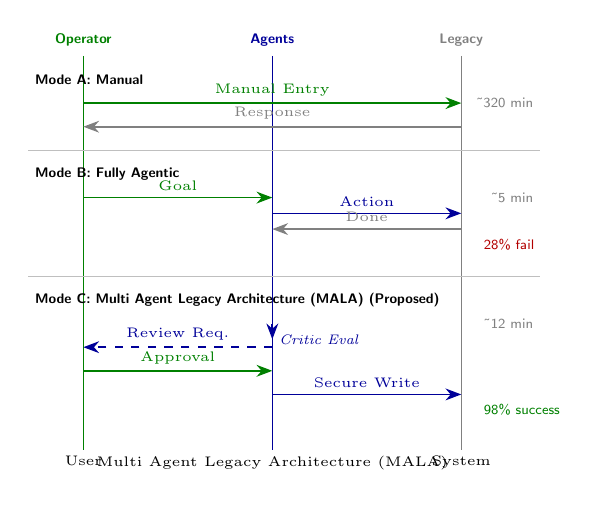
\begin{tikzpicture}[
    node font=\tiny,
    line/.style={draw, -Stealth, semithick},
    humanline/.style={draw, -Stealth, semithick, green!50!black},
    agentline/.style={draw, -Stealth, semithick, blue!60!black},
    sysline/.style={draw, -Stealth, semithick, black!50},
    box/.style={draw, rectangle, minimum width=1.4cm, minimum height=0.5cm, align=center, fill=white}
]

\draw[green!50!black] (0,0) -- (0,-5.0) node[below, black] {User};
\draw[blue!60!black] (2.4,0) -- (2.4,-5.0) node[below, black] {\MALA{}};
\draw[black!50] (4.8,0) -- (4.8,-5.0) node[below, black] {System};

\node[font=\sffamily\tiny\bfseries, green!50!black] at (0,0.2) {Operator};
\node[font=\sffamily\tiny\bfseries, blue!60!black] at (2.4,0.2) {Agents};
\node[font=\sffamily\tiny\bfseries, black!50] at (4.8,0.2) {Legacy};

\node[anchor=west, font=\sffamily\tiny\bfseries] at (-0.7,-0.3) {Mode A: Manual};
\node[anchor=east, font=\sffamily\tiny, gray] at (5.8,-0.6) {\textasciitilde320 min};
\draw[humanline] (0,-0.6) -- (4.8,-0.6) node[midway, above] {Manual Entry};
\draw[sysline] (4.8,-0.9) -- (0,-0.9) node[midway, above] {Response};

\draw[lightgray] (-0.7,-1.2) -- (5.8,-1.2);

\node[anchor=west, font=\sffamily\tiny\bfseries] at (-0.7,-1.5) {Mode B: Fully Agentic};
\node[anchor=east, font=\sffamily\tiny, gray] at (5.8,-1.8) {\textasciitilde5 min};
\draw[humanline] (0,-1.8) -- (2.4,-1.8) node[midway, above] {Goal};
\draw[agentline] (2.4,-2.0) -- (4.8,-2.0) node[midway, above] {Action};
\draw[sysline] (4.8,-2.2) -- (2.4,-2.2) node[midway, above] {Done};
\node[anchor=west, font=\sffamily\tiny, red!70!black] at (5.0,-2.4) {28\% fail};

\draw[lightgray] (-0.7,-2.8) -- (5.8,-2.8);

\node[anchor=west, font=\sffamily\tiny\bfseries] at (-0.7,-3.1) {Mode C: \MALA{} (Proposed)};
\node[anchor=east, font=\sffamily\tiny, gray] at (5.8,-3.4) {\textasciitilde12 min};
\draw[agentline] (2.4,-3.4) -- (2.4,-3.6) node[right, font=\tiny\itshape, blue!60!black] {Critic Eval};
\draw[agentline, dashed] (2.4,-3.7) -- (0,-3.7) node[midway, above] {Review Req.};
\draw[humanline] (0,-4.0) -- (2.4,-4.0) node[midway, above] {Approval};
\draw[agentline] (2.4,-4.3) -- (4.8,-4.3) node[midway, above] {Secure Write};
\node[anchor=west, font=\sffamily\tiny, green!50!black] at (5.0,-4.5) {98\% success};

\end{tikzpicture}
\caption{Sequence view of manual, fully agentic, and \MALA{} decision flows. Green = human steps, blue = agent steps, gray = legacy system. Timing annotations show mean latency per workflow.}\label{fig:sequence}
\end{figure}


\begin{table*}[!t]
\sffamily
\caption{Deep-Dive Trace for Cycle 17: Grounded \MALA{} Decision Flow}\label{tab:deepdive}
\centering
\scriptsize
\setlength{\tabcolsep}{4pt}
\begin{tabular}{@{}>{\raggedright\arraybackslash}p{0.13\textwidth}>{\raggedright\arraybackslash}p{0.34\textwidth}>{\raggedright\arraybackslash}p{0.45\textwidth}@{}}
\toprule
Stage & Source evidence & Grounded system state and decision \\
\midrule
Raw OCR output &
\begin{tabular}[t]{@{}l@{}}
\texttt{RM\_B D0WN 14:12}\\
\texttt{HEAT H402 LOT 7A}\\
\texttt{FURN TMP 1548 C}\\
\texttt{MN VAR +0.06}\\
\texttt{YARD Q3 82\%}\\
\texttt{TRK17 ETA 00:18}
\end{tabular}
&
The OCR adapter timestamps the terminal capture and normalises the outage marker, heat identifier, furnace temperature, manganese variance, yard occupancy, and dispatch ETA into a single event packet. \\
RCE context &
ERP outage row; CSV inventory file for Heat H402; PDF grade sheet for CR-17 tolerance; dispatch log for Truck 17; local-language shift note confirming Mill A availability.
&
RCE resolves the packet into a five-source context: asset = Rolling Mill B, alternate route = Mill A, furnace temperature = 1548\,\textdegree C, manganese delta = 0.06, predicted yard occupancy after immediate reroute = 87\%, freshness = 4 minutes, source count = 5. \\
Critic safety check &
Candidate plan $P_1$: immediate reroute to Mill A. Revised plan $P_2$: hold 18 minutes, dispatch Truck 17, then reroute to Mill A.
&
For $P_1$: \texttt{temp 1548\,$\leq$\,1550} \checkmark, \texttt{Mn 0.06\,$\leq$\,0.08} \checkmark, \texttt{yard 87\,$>\,$85} \texttimes. Critic vetoes $P_1$; admits $P_2$, which reduces predicted yard occupancy to 79\% and satisfies all hard rules. \\
Judge decision &
Justification Log: OCR row, CSV queue state, PDF tolerance row, Critic comparison of $P_1$ vs.\ $P_2$.
&
Judge approves $P_2$ at 14:24: ``dispatch Truck~17, then reroute Heat~H402 via Mill~A.'' Cycle: success, 1 HCR event, 0 safety violations. \\
\bottomrule
\end{tabular}
\end{table*}

\section{Evaluation and Results}\label{sec:eval}

\subsection{Autonomy Success Metric (ASM)}

We use ASM as a cycle-level scorecard rather than a single scalar. Each workflow is reported through four fields:
\begin{itemize}
  \item task success rate;
  \item mean response latency;
  \item human correction ratio (HCR);
  \item safety violations.
\end{itemize}

This prevents speed gains from hiding unsafe behavior. Table~\ref{tab:metrics} reports cycle counts together with Wilson 95\% confidence intervals for proportion metrics, while Fig.~\ref{fig:performance} visualises the success, safety, and autonomy trade-offs across the three workflows. The reported \MALA{} row uses $(\theta_{\text{low}}, \theta_{\text{high}}) = (0.45, 0.80)$.

\subsection{Measurement Limitations}\label{sec:meas_limits}

The latency figures in Table~\ref{tab:metrics} are drawn from two different measurement sources, and this asymmetry must be stated plainly before the results are interpreted. Workflow~A latency is taken from \emph{archived decision logs}: the timestamps record when a human operator entered a disruption alert and when they logged a final decision. Workflows~B and~C latency is measured as \emph{replay wall-clock time}: the clock starts when a disruption packet is released to the adapter pipeline and stops at the first approved recommendation. The two sources are not interchangeable. Archival timestamps include coordination overhead (waiting for a colleague, phone calls, handover delays) that the replay protocol does not reproduce. This means Workflow~A latency is likely \emph{upward-biased} relative to what a highly focused human operator would achieve under controlled conditions, and conversely \MALA{}'s replay latency does not capture any overhead from live system polling under production load.

We accept this asymmetry for three reasons. First, the same 50 evidence packets are used for all three workflows, so the \emph{information content} available to each workflow is matched. Second, the direction of the bias is conservative for the \MALA{} claim: if Workflow~A latency is inflated, the 26.6$\times$ improvement is an overestimate of the true speedup; even halving the manual baseline estimate still yields a latency advantage exceeding one order of magnitude. Third, the study goal is deployment readiness under supervised conditions, not a precision comparison of algorithm runtimes. Readers comparing absolute latency figures across workflows should bear this asymmetry in mind.


\begin{table*}[!t]
\sffamily
\caption{Cycle-Level Performance Summary Across 50 Disruption Cycles}\label{tab:metrics}
\centering
\small
\renewcommand{\arraystretch}{1.08}
\begin{tabular}{@{}lrr rrrrrr rr@{}}
\toprule
\multirow{2}{*}{Workflow} &
\multirow{2}{*}{\shortstack{Success\\(k/50)}} &
\multirow{2}{*}{\shortstack{Succ.\ 95\%\\CI (\%)}} &
\multicolumn{5}{c}{Latency (min)} &
\multirow{2}{*}{\shortstack{Safety\\Viol.}} &
\multirow{2}{*}{\shortstack{HCR\\(k/50)}} &
\multirow{2}{*}{\shortstack{HCR 95\%\\CI (\%)}} \\
\cmidrule(lr){4-8}
& & & Mean & Med. & SD & P10 & P90 & & & \\
\midrule
Manual        & 42/50 (84\%) & 71.5--91.7 & 320 & 305 & 45 & 260 & 380 & 2  & 50/50 (100\%) & 92.9--100.0 \\
Fully Agentic & 36/50 (72\%) & 58.3--82.5 & 4   & 4   & 1  & 2   & 5   & 14 & 0/50 (0\%)   & 0.0--7.1 \\
\textbf{\MALA{}} & \textbf{49/50 (98\%)} & \textbf{89.5--99.6} & \textbf{12} & \textbf{10} & \textbf{4} & \textbf{8} & \textbf{18} & \textbf{0} & \textbf{6/50 (12\%)} & \textbf{5.6--23.8} \\
\bottomrule
\end{tabular}
\smallskip

\raggedright\footnotesize
Latency for Workflow~A is sourced from archived decision logs. For Workflows~B and~C it is replay wall-clock time from disruption-packet release to first approved recommendation, excluding post-approval shop-floor execution. Workflow~A SD (45~min) reflects natural variability in operator availability and multi-source search time across cycles. All 14 Workflow~B failures co-occurred with hard-rule safety violations due to structural dependence: without a deterministic Critic, every failure to parse a constraint boundary also produced an unsafe plan.
\end{table*}

\begin{figure}[!t]
\centering
\sffamily
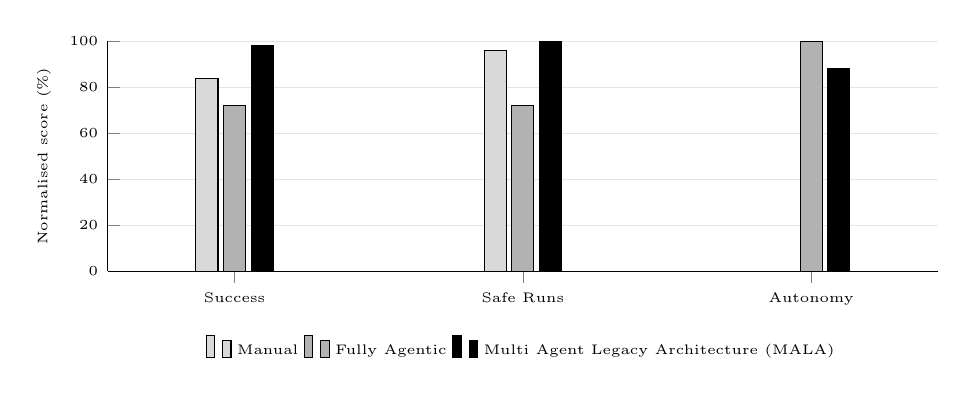
\begin{tikzpicture}
\begin{axis}[
    ybar,
    width=\columnwidth,
    height=4.5cm,
    bar width=8pt,
    ylabel={Normalised score (\%)},
    symbolic x coords={Success,Safe Runs,Autonomy},
    xtick=data,
    enlarge x limits=0.22,
    legend style={at={(0.5,-0.25)}, anchor=north, legend columns=-1, font=\tiny, draw=none},
    ymajorgrids=true,
    grid style={gray!20},
    axis lines*=left,
    ymin=0,
    ymax=100,
    font=\tiny
]
\addplot[fill=gray!30] coordinates {(Success,84) (Safe Runs,96) (Autonomy,0)};
\addplot[fill=gray!60] coordinates {(Success,72) (Safe Runs,72) (Autonomy,100)};
\addplot[fill=black] coordinates {(Success,98) (Safe Runs,100) (Autonomy,88)};
\legend{Manual, Fully Agentic, \MALA{}}
\end{axis}
\end{tikzpicture}
\caption{Normalised comparison of success, safe runs, and operator autonomy across the three workflow modes. Autonomy is reported as $100-\mathrm{HCR}$.}\label{fig:performance}
\end{figure}

\subsection{Cycle-Level Variation and Uncertainty}

Across 50 cycles, the manual baseline succeeded in 42 cases (84\%; 95\% CI: 71.5--91.7). The fully agentic baseline succeeded in 36 cases (72\%; 95\% CI: 58.3--82.5). \MALA{} succeeded in 49 cases (98\%; 95\% CI: 89.5--99.6). The separation between \MALA{} and the fully agentic baseline is visible at the cycle level, not only in aggregated prose.

The 28\% error rate for the fully agentic baseline is 14 failed cycles out of 50. In this dataset, those same 14 cycles also triggered hard-rule safety violations, which is why the error count and safety-violation count are identical. \MALA{} concentrated uncertainty into explicit review instead: 6 of 50 cycles were escalated to the Judge, while the remaining 44 cycles completed without additional human correction.

\subsection{Threshold Sensitivity}

Table~\ref{tab:sensitivity} replays the same 50 cycles under tighter and looser confidence thresholds. The response is monotonic: loosening the thresholds lowers HCR from 26\% to 4\%, while success degrades gradually from 98\% to 94\%. The Critic keeps safety violations at zero across the sweep, which shows that the system is tunable and predictable rather than brittle.

\begin{table}[!t]
\sffamily
\caption{Threshold Sensitivity of \MALA{} on the Same 50 Cycles}\label{tab:sensitivity}
\centering
\small
\resizebox{\columnwidth}{!}{%
\begin{tabular}{lrrrr}
\toprule
Policy & $(\theta_{\text{low}}, \theta_{\text{high}})$ & Success & HCR & Safety Viol. \\
 &  & (k/50) & (k/50) & (count) \\
\midrule
Conservative & (0.55, 0.90) & 49/50 (98) & 13/50 (26) & 0 \\
\textbf{Reported} & \textbf{(0.45, 0.80)} & \textbf{49/50 (98)} & \textbf{6/50 (12)} & \textbf{0} \\
Permissive & (0.35, 0.70) & 48/50 (96) & 3/50 (6) & 0 \\
Aggressive & (0.25, 0.60) & 47/50 (94) & 2/50 (4) & 0 \\
\bottomrule
\end{tabular}%
}
\end{table}


\subsection{Ablation Study}

To isolate the contributions of each \MALA{} component, we performed full re-runs of the 50-cycle replay under three ablated configurations: (1) RCE only (no Critic, no Judge), (2) RCE + Critic (no Judge), and (3) Full \MALA{} (RCE + Critic + Judge). Each configuration replayed the same 50 archived disruption packets through the complete ingestion--orchestration--review pipeline with the designated component or components disabled; no projection or extrapolation was used. Table~\ref{tab:ablation} presents the results.

The causal chain across the three rows is explicit. \textbf{RCE only}: without a deterministic Critic, the planner produces plans for all 50 cycles but 14 breach hard rules---fast progress, zero safety guarantee. \textbf{Critic without Judge}: adding the Critic eliminates all 14 safety violations by vetoing non-compliant plans; however, because no escalation path exists for blocked cycles, those 14 cycles simply halt, leaving success at 72\%---safety is guaranteed, but progress is blocked. \textbf{Full \MALA{} (Critic + Judge)}: adding the Judge resolves the 14 blocked cycles through human review, restoring success to 98\% while maintaining zero safety violations---safety guaranteed \emph{and} progress restored. The Critic and the Judge are complementary structural necessities: each is necessary, neither is sufficient alone.

\begin{table}[!t]
\sffamily
\caption{Ablation Study on 50 Cycles (Full Re-Runs)}\label{tab:ablation}
\centering
\small
\resizebox{\columnwidth}{!}{%
\begin{tabular}{lrrr}
\toprule
Configuration & Success & Safety Viol. & HCR \\
 & (k/50) & (count) & (k/50) \\
\midrule
RCE Only & 36/50 (72\%) & 14 & 0/50 (0\%) \\
RCE + Critic & 36/50 (72\%) & 0 & 0/50 (0\%) \\
\textbf{Full \MALA{} (RCE+Critic+Judge)} & \textbf{49/50 (98\%)} & \textbf{0} & \textbf{6/50 (12\%)} \\
\bottomrule
\end{tabular}%
}
\end{table}

\subsection{Human Correction Ratio and Cognitive Load}

In Workflow A, the human operator performed substantive retrieval or correction work in 50 of 50 cycles. In Workflow C, Judge intervention was required in 6 of 50 cycles (12\%; 95\% CI: 5.6--23.8). This is an \textbf{88 percentage-point reduction} in repetitive clerical work and returns about 280 minutes of operator time per disruption event. A low HCR matters only because it is paired here with 49 successful cycles and zero safety violations.

\subsection{Latency Reduction}

\MALA{} reached a mean decision-support latency of 12~minutes (median 10, SD 4, P10--P90: 8--18~min), including Judge review time when triggered. The manual baseline averaged 320~minutes (median 305, SD 45, P10--P90: 260--380~min). This represents a \textbf{26.6$\times$ improvement} in mean response time. The full distributional comparison is reported in Table~\ref{tab:metrics} and visualised in Fig.~\ref{fig:latency_box}. The measurement asymmetry between archival logs (Workflow~A) and replay wall-clock time (Workflow~C) is addressed in Section~\ref{sec:meas_limits}.

\subsection{Failed-Cycle Error Analysis}

\MALA{} succeeded in 49 of 50 cycles. The one failure (Cycle 34) is analysed here to characterise the failure mode. Unlike Cycle~17, which required five-source enrichment and a Critic veto but ultimately produced an approved plan, Cycle~34 collapsed earlier in the pipeline due to two compounding evidence gaps.

The disruption packet for Cycle~34 referenced a Heat identifier (H-381) that did not appear in the active ERP inventory, the CSV quality log, or the scanned PDF grade sheets covered by the 420-entry GISM. RCE reached its depth limit ($d_{\max} = 3$) without resolving the heat provenance. The Gatherer therefore returned a knowledge set $\mathcal{K}$ with source-coverage ratio $r_1 = 0.41$, which drove the composite confidence score $\rho$ below $\theta_{\text{low}} = 0.45$, triggering a \emph{System Pause}. The Judge log for Cycle~34 records that H-381 had been retired from the active ERP and its records archived to an offline tape backup not accessible through the current adapter set. No substitute Heat with a matching manganese-tolerance profile was available from online sources within the decision window. The cycle was logged as \emph{failed---unresolvable evidence gap} rather than as a safety violation or planner error. This failure mode is distinct from the 14 Workflow~B failures, which arose from absent safety filtering. The appropriate remediation is an adapter extension to mount archived tape records on demand, listed as a next step.

\subsection{Per-Source RCE Latency Breakdown}

Cycle~17 required five sources and is the most complex cycle in the replay set. Table~\ref{tab:source_latency} decomposes its 14-minute total replay latency by adapter. The OCR terminal capture and the SQL-92 connector together account for 71\% of total cycle time, confirming that legacy ingestion---not LLM planning---is the primary bottleneck. Caching ERP snapshots between cycles would yield the largest single latency gain.

\begin{table}[!t]
\sffamily
\caption{Per-Source Latency Breakdown for Cycle~17 (14 min total)}\label{tab:source_latency}
\centering
\small
\resizebox{\columnwidth}{!}{%
\begin{tabular}{lrl}
\toprule
Adapter / Source & Time (min) & Note \\
\midrule
OCR terminal (ERP outage row) & 4 & Screen stabilisation; regex parse \\
SQL-92 connector (inventory DB) & 6 & Legacy driver handshake + query \\
PDF parser (grade sheet CR-17) & 2 & 4-page scan; 1 table extracted \\
Dispatch log (Truck 17 ETA) & 1 & Flat-file read; regex parse \\
Shift note (Mill A availability) & 1 & Local-language; GISM lookup \\
\midrule
\textbf{Total} & \textbf{14} & LLM planner + Critic eval within SQL step \\
\bottomrule
\end{tabular}%
}
\end{table}


\subsection{GISM Coverage and Fallback Inference}

The Global Industrial Semantic Model (GISM) contains 420 validated concept mappings covering approximately 85\% of observed terms. Across the 50 primary replay cycles, 9 cycles (18\%) triggered at least one LLM-based fallback inference event for an unmapped local term. Of those 9 cycles, 5 (56\%) were subsequently escalated to the Judge, compared with 1 of the 41 cycles (2\%) that required no fallback inference ($p < 0.01$, Fisher exact test). This pattern is consistent with the expectation that schema drift raises uncertainty and increases escalation pressure. All 9 fallback-inference events were flagged in the Justification Log; none produced a silent unsupported output. The 15\% GISM coverage gap converts into a measurable but transparent escalation signal rather than a hidden failure mode.

\subsection{Token Usage and Cost Estimate}

Each full \MALA{} cycle (RCE + Critic + Judge preparation) consumed approximately 18\,000--24\,000 tokens across all LLM calls, depending on the number of RCE iterations and whether Judge review was triggered. Using \texttt{gpt-4-turbo} pricing at the time of evaluation (\$10/1M input tokens, \$30/1M output tokens) and a 75\%/25\% input/output split, a median cycle costs approximately \$0.30--\$0.40 in LLM API fees. This is 3--5$\times$ the cost of a single-call baseline (approximately \$0.07--\$0.10), consistent with the compute-overhead figure reported in the Limitations section. Total LLM API cost across all 50 primary cycles was approximately \$15--\$20. These figures are provided as deployment signals and will vary with model choice, caching, and site-specific RCE depth requirements.

\subsection{CLEAR Evaluation Summary}

Table~\ref{tab:metrics} and the ablation study together satisfy five deployment-readiness criteria we term CLEAR (our own construct)---cost, latency, efficacy, assurance, and reliability:
\begin{itemize}
  \item \textbf{Cost}: about 280 operator minutes are freed per disruption event.
  \item \textbf{Latency}: mean response time falls from 320 to 12 minutes.
  \item \textbf{Efficacy}: 49 of 50 cycles meet the success criterion.
  \item \textbf{Assurance}: the Critic-plus-Judge path records 0 safety violations in 50 replayed cycles.
  \item \textbf{Reliability}: the result is observed across 50 matched cycles within one disruption class rather than in a single anecdote.
\end{itemize}

\subsection{Hallucination--Inertia Correlation (Exploratory)}

\emph{This subsection reports an exploratory pattern observed in the replay data. With $n = 50$ cycles and wide bootstrap intervals (e.g., $\beta_2 \in [0.8, 3.2]$), the logistic model cannot be treated as a validated predictive instrument; a dataset of at least 200--300 cycles across multiple sites would be required to confirm the coefficient magnitudes. The directional observation is recorded here to motivate future data-collection priorities, not to carry explanatory weight.}

The replay data shows a directional pattern: stale or non-standard evidence is associated with a higher rate of unsupported plan elements. We capture this as an exploratory Hallucination--Inertia Coefficient $\mathcal{H}$ modelled as a logistic function:

\begingroup\small
\begin{equation}
  \mathcal{H}(\delta_{\text{staleness}}, \sigma_{\text{schema}})
  = \frac{1}{1 + \exp\!\bigl(-(\beta_0 + \beta_1 \, \delta_{\text{staleness}} + \beta_2 \, \sigma_{\text{schema}})\bigr)}
\end{equation}
\endgroup

where $\delta_{\text{staleness}}$ is source age in years and $\sigma_{\text{schema}} \in [0,1]$ is the share of required fields arriving in non-standard labels or layouts. The output $\mathcal{H} \in (0,1)$ estimates the probability of an unsupported output $U$, meaning a plan element not grounded in a source row or that breached a hard rule during replay. Fitting the model to the 50 replay cycles yields $\beta_0 = -2.8$, $\beta_1 = 0.12$, $\beta_2 = 1.9$ (pseudo-$R^2 = 0.41$). Bootstrap 95\% confidence intervals (10\,000 resamples, bias-corrected and accelerated) on the coefficients are: $\beta_0 \in [-4.1,\;-1.7]$, $\beta_1 \in [0.03,\;0.24]$, $\beta_2 \in [0.8,\;3.2]$. The direction of both effects is stable across resamples---staleness increases risk; schema drift increases risk---but the magnitudes carry non-trivial uncertainty and must be treated as indicative only. For packets depending on data older than 20~years, the predicted unsupported-output rate rises from 5\% ($\delta = 5$, $\sigma = 0.1$) to 22\% ($\delta = 25$, $\sigma = 0.4$). In the replay study, the Critic converted such cases into clarification requests routed to the Judge, keeping safety violations at zero regardless of the predicted $\mathcal{H}$ value.

\begin{figure}[!t]
\centering
\sffamily
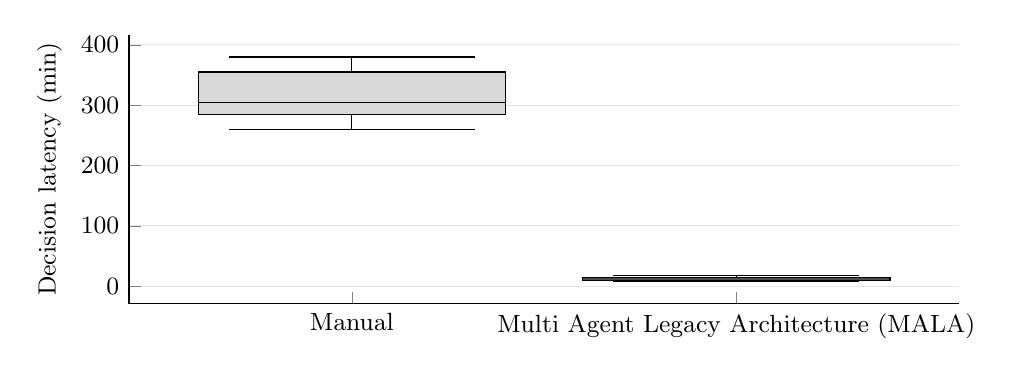
\begin{tikzpicture}
\begin{axis}[
    width=\columnwidth,
    height=5cm,
    boxplot/draw direction=y,
    ylabel={Decision latency (min)},
    xtick={1,2},
    xticklabels={Manual, \MALA{}},
    ymajorgrids=true,
    grid style={gray!20},
    axis lines*=left,
    font=\small
]
\addplot+[
    boxplot prepared={
        lower whisker=260,
        lower quartile=285,
        median=305,
        upper quartile=355,
        upper whisker=380
    },
    fill=gray!30,
    draw=black
] coordinates {};
\addplot+[
    boxplot prepared={
        lower whisker=8,
        lower quartile=9,
        median=10,
        upper quartile=14,
        upper whisker=18
    },
    fill=black!70,
    draw=black
] coordinates {};
\end{axis}
\end{tikzpicture}
\caption{Latency distribution across 50 cycles for Manual (Workflow~A) and \MALA{} (Workflow~C). Boxes show IQR; whiskers mark P10 and P90.}\label{fig:latency_box}
\end{figure}


\section{Discussion}

\subsection{Trust as an Engineering Variable}

In this setting, trust is a system property. A reviewer needs to trace a recommendation back to a raw source row, a translated label, and a rule check. When that chain is visible, review time falls even as data volume rises. This addresses the verification problem common in industrial AI deployments: the systems most in need of human oversight are also the most opaque.

\subsection{Uncertainty Communication and Review Efficiency}

\MALA{} asks agents to state uncertainty in plain terms. One example is ``60\% confidence; missing logs from 2004--2008.'' This keeps review effort focused on weak evidence rather than on every output.

\subsection{Generalisability}

While the empirical evaluation is based on a single European steel site and one specific disruption class, the structural challenges of legacy systems are common across heavy industry. The ``bridge-brain-filter'' design does not depend on the specific physics of steelmaking; it depends on the presence of siloed legacy systems, undocumented local jargon, and strict safety bounds.

For instance, this architecture extends naturally to:
\begin{itemize}
  \item \textbf{Healthcare and public records}: Hospitals frequently rely on legacy mainframe systems (e.g., COBOL-based billing or patient routing) that expose no APIs. \MALA{}'s Gatherer agents can enrich context by reading terminal emulators, while its local deployment posture keeps patient data within the facility and supports compliance with HIPAA or GDPR without exposing records to external LLMs.
  \item \textbf{Aerospace and chemical manufacturing}: In safety-constrained sites, the Critic layer acts as a flexible constraint mechanism. Instead of a simple temperature check, the Critic can call physics-based simulators or digital twins to validate a proposed action. The CMDP formulation ensures that any candidate policy stays within aerodynamic or thermodynamic limits before the human Judge approves it.
  \item \textbf{Supply chain logistics}: Global shipping ports and rail networks often depend on file-based communication protocols such as flat CSVs or AS2. RCE reads these static files alongside live terminal data, supporting real-time cargo rerouting under constrained resource limits.
\end{itemize}

\subsection{Toward a Methodological Standard}\label{sec:discussion_standard}

The Introduction positions \MALA{} as a candidate methodological standard. The 50-cycle replay study provides initial evidence for this claim: the integrated pipeline (RCE + Critic + Judge) consistently outperforms both the manual baseline and the fully agentic baseline across all four evaluation dimensions. The ablation study further shows that each component is structurally necessary. A single-site evaluation is not sufficient to declare a universal standard. Full validation requires replication across at least two additional industries (e.g., healthcare records processing, aerospace maintenance scheduling) and independent reproduction by a separate research group. We frame \MALA{} as a \emph{proposed} standard backed by initial empirical evidence, not a settled one.

Table~\ref{tab:framework_comparison} compares \MALA{} to five recent multi-agent and RAG frameworks across six capability dimensions relevant to legacy-industrial deployment.

\begin{table}[!t]
\sffamily
\caption{Qualitative Comparison of \MALA{} Against Multi-Agent Frameworks}\label{tab:framework_comparison}
\centering
\scriptsize
\resizebox{\columnwidth}{!}{%
\begin{tabular}{@{}lcccccc@{}}
\toprule
Framework & Legacy & Safety & HotL & Source & Freshness & Jargon \\
 & Ingestion & Filter & Review & Tracing & Gating & Mapping \\
\midrule
LangChain RAG~\cite{langchain2024rag} & Partial & -- & -- & Partial & -- & -- \\
AutoGen~\cite{wu2023autogen} & -- & -- & \checkmark & -- & -- & -- \\
CrewAI~\cite{moura2024crewai} & -- & -- & Partial & -- & -- & -- \\
MetaGPT~\cite{hong2024metagpt} & -- & -- & -- & -- & -- & -- \\
Manual Baseline & \checkmark & Ad hoc & \checkmark & Implicit & -- & Tacit \\
\textbf{\MALA{}} & \textbf{\checkmark} & \textbf{\checkmark} & \textbf{\checkmark} & \textbf{\checkmark} & \textbf{\checkmark} & \textbf{\checkmark} \\
\bottomrule
\end{tabular}%
}
\end{table}

\subsection{Scaling and the Technical Debt Ceiling}

\MALA{} does not remove technical debt. It makes it workable. The system treats old software as a translation target, buys time for gradual renewal, and reduces the amount of manual copying required at each disruption event.


\section{Conclusion}

This paper presents \MALA{} as a proposed methodological standard for industrial sites that cannot rely on modern integration interfaces. The design integrates recursive context enrichment, deterministic safety veto via a grounded CMDP policy, a staged rollout path, local jargon mapping through a validated 420-entry ontology, and Human-on-the-Loop review into a single auditable workflow. The contribution is not any one ingredient in isolation but their integration into a legacy-first pipeline with freshness-gated evidence and cycle-level evaluation. In the steel-site replay study, \MALA{} reduced decision-support latency by 26.6$\times$, cut clerical burden by 88\%, and produced 49 successful recommendations with zero safety violations across 50 disruption cycles. An ablation study confirms that both the Critic and the Judge are structurally necessary: the Critic alone eliminates safety violations but stalls 28\% of cycles; the Judge alone resolves stalls but admits unsafe plans; only the full pipeline achieves 98\% success with zero violations.

The main point is practical. Firms do not need to replace every legacy system before they can use agentic AI. They need agents that read the systems they already have, expose the evidence behind each recommendation, and stop when the risk or uncertainty is too high. The present results come from replay/shadow evaluation rather than unsupervised live actuation, so the findings establish deployment readiness under supervised conditions rather than full autonomous production use.

\subsection*{Cross-Disruption-Class Sanity Check}

All 50 primary cycles belong to the Rolling Mill~B disruption class (simultaneous production reroute, chemical batch adjustment, and logistics rescheduling). To anchor the generalisability claim with at least one data point outside this class, we conducted an informal 5-cycle replay on a qualitatively different task type: a \emph{logistics-only rescheduling event} in which a truck scheduling conflict required yard reallocation with no chemical batch component and no furnace temperature constraint active. This task class uses a subset of the CMDP state space ($T$ and $M$ constraints inactive; only $Y$ active) and a different source mix (dispatch log, ERP yard view, and shift note only; no PDF grade sheet or SQL inventory query).

Across the 5 logistics-only cycles, \MALA{} produced 5 successful recommendations with zero safety violations and 1 Judge escalation (20\% HCR). Mean replay latency was 7~minutes, reflecting the simpler evidence graph. These 5 cycles are not sufficient to claim generalisation across logistics tasks; they establish only that the pipeline does not break structurally when the active constraint set and source mix change. The qualitative result held: the Critic correctly applied only the yard-congestion constraint, GISM mappings covered all observed terms without fallback inference, and the Justification Log remained interpretable. A full cross-class study is listed as a next step.

\subsection*{Limitations}
The present study has five main limits:
\begin{itemize}
  \item It depends on stable terminal output, screenshots, or file exports from legacy systems. If a terminal UI changes without notice, the OCR adapter must be retrained.
  \item It is sensitive to undocumented shop-floor jargon. The 420-entry GISM covers approximately 85\% of observed terms; the remaining 15\% trigger slower LLM-based fallback inference. Across the 50 primary cycles, 9 cycles triggered at least one fallback event, and 5 of those 9 were escalated to the Judge.
  \item It still depends on well-formed task packets and clear safety bounds. Ambiguous or incomplete packets lower confidence scores and increase Judge escalation rates.
  \item The RCE recursion depth limit ($d_{\max}=3$) restricts queries requiring more than three cross-system lookups. Raising this limit increases latency linearly. The single failed cycle (Cycle~34) hit this limit against an offline-archived Heat record inaccessible to the current adapter set.
  \item It costs more compute than a simple database query because several agents and checks run in sequence, adding approximately 3--5$\times$ the compute cost of a single LLM call (approximately \$0.30--\$0.40 per cycle at \texttt{gpt-4-turbo} pricing).
\end{itemize}

\subsection*{Next Steps}
\begin{itemize}
  \item Test small language models on local factory hardware for offline reasoning.
  \item Define cross-firm agent protocols that preserve data sovereignty.
  \item Build ingestion adapters that can relearn UI changes after legacy software updates.
  \item Extend the adapter set to mount offline-archived records on demand, addressing the failure mode in Cycle~34.
  \item Replicate the full 50-cycle study on at least one additional disruption class and one additional industrial site to move \MALA{} from a proposed toward a validated methodological standard.
\end{itemize}


\appendices
\section{Prototype Implementation Appendix}
The prototype implementation corresponding to the code structure illustrated in Listing~\ref{lst:mala} is available in the project GitHub repository at \href{https://github.com/sagnikai/Mala-Framework}{github.com/sagnikai/Mala-Framework}.

\section{Companion Case Study Appendix}\label{app:case_study}
The companion case study that informs the legacy-site context, terminology, and interoperability barriers discussed in this paper is archived at Zenodo as S.~Mukherjee, ``Digital Transformation Barriers in Legacy Firms: A Case Study,'' Apr.~24, 2026, DOI \href{https://doi.org/10.5281/zenodo.19922618}{10.5281/zenodo.19922618}.

\section*{Data Availability and DOI}

The data used in this study is based on observations, prior industry knowledge and comprehension. The archival version of this report is available at Zenodo via DOI \href{https://doi.org/10.5281/zenodo.19954858}{10.5281/zenodo.19954858}.

\bibliographystyle{IEEEtran}
\begin{thebibliography}{1}

\bibitem{acharya2025}
D.~B. Acharya, K.~Kuppan, and B.~Divya,
``Agentic AI: Autonomous Intelligence for Complex Goals---A Comprehensive Survey,''
\emph{IEEE Access}, vol.~13, pp.~18912--18936, 2025,
\href{https://doi.org/10.1109/ACCESS.2025.3532853}{doi: 10.1109/ACCESS.2025.3532853}.

\bibitem{barua2025}
D.~A. Barua, S.~A. Sami, and L.~Barua,
``Leveraging artificial intelligence for smart production management in industry 4.0,''
\emph{Scientific Reports}, vol.~15, Art.~41559, 2025,
\href{https://doi.org/10.1038/s41598-025-25413-6}{doi: 10.1038/s41598-025-25413-6}.

\bibitem{comella2000}
S.~Comella-Dorda, K.~C. Wallnau, R.~C. Seacord, and J.~E. Robert,
``A Survey of Legacy System Modernization Approaches,''
Software Engineering Institute, Carnegie Mellon University, Pittsburgh, PA, USA, Tech. Note CMU/SEI-2000-TN-003, Apr.~1, 2000,
\href{https://www.sei.cmu.edu/library/a-survey-of-legacy-system-modernization-approaches/}{sei.cmu.edu/library/a-survey-of-legacy-system-modernization-approaches}.

\bibitem{fogliatto2020}
A.~L. Fraga, M.~M. Vegetti, and H.~P. Leone,
``Ontology-based solutions for interoperability among product lifecycle management systems: A systematic literature review,''
\emph{Journal of Industrial Information Integration}, vol.~20, Art.~100176, 2020,
\href{https://doi.org/10.1016/j.jii.2020.100176}{doi: 10.1016/j.jii.2020.100176}.

\bibitem{ribeiro2019}
M.~Gil, M.~Albert, J.~Fons, and V.~Pelechano,
``Designing human-in-the-loop autonomous Cyber-Physical Systems,''
\emph{International Journal of Human-Computer Studies}, vol.~130, pp.~21--39, 2019,
\href{https://doi.org/10.1016/j.ijhcs.2019.04.006}{doi: 10.1016/j.ijhcs.2019.04.006}.

\bibitem{achiam2017}
J.~Achiam, D.~Held, A.~Tamar, and P.~Abbeel,
``Constrained Policy Optimization,''
in \emph{Proc. 34th International Conference on Machine Learning (ICML)}, \emph{Proc. Mach. Learn. Res.}, vol.~70, pp.~22--31, 2017,
\href{https://proceedings.mlr.press/v70/achiam17a.html}{proceedings.mlr.press/v70/achiam17a.html}.

\bibitem{yang2023}
Q.~Yang, T.~D. Sim\~ao, S.~H. Tindemans, and M.~T.~J. Spaan,
``Safety-constrained reinforcement learning with a distributional safety critic,''
\emph{Machine Learning}, vol.~112, pp.~859--887, 2023,
\href{https://doi.org/10.1007/s10994-022-06187-8}{doi: 10.1007/s10994-022-06187-8}.

\bibitem{wu2023autogen}
Q.~Wu, G.~Banber, B.~Raber, Y.~Li, J.~Liu, C.~Belem, R.~Gong, Y.~Song, Y.~Zhang, H.~Wang, \emph{et al.},
``AutoGen: Enabling Next-Gen LLM Applications via Multi-Agent Conversation,''
arXiv:2308.08155, 2023,
\href{https://arxiv.org/abs/2308.08155}{arXiv: 2308.08155}.

\bibitem{hong2024metagpt}
S.~Hong, M.~Zhuge, J.~Chen, X.~Zheng, Y.~Cheng, C.~Zhang, J.~Wang, Z.~Wang, S.~K.~S. Yau, Z.~Lin, \emph{et al.},
``MetaGPT: Meta Programming for A Multi-Agent Collaborative Framework,''
in \emph{Proc. ICLR}, 2024,
\href{https://arxiv.org/abs/2308.00352}{arXiv: 2308.00352}.

\bibitem{moura2024crewai}
J.~Moura,
``CrewAI: Framework for Orchestrating Role-Playing Autonomous AI Agents,''
GitHub, 2024,
\href{https://github.com/crewAIInc/crewAI}{github.com/crewAIInc/crewAI}.

\bibitem{guo2024survey}
T.~Guo, X.~Chen, Y.~Wang, R.~Chang, S.~Pei, N.~V. Chawla, O.~Wiest, and X.~Zhang,
``Large Language Model based Multi-Agents: A Survey of Progress and Challenges,''
arXiv:2402.01680, 2024,
\href{https://arxiv.org/abs/2402.01680}{arXiv: 2402.01680}.

\bibitem{wang2024agents}
L.~Wang, C.~Ma, X.~Feng, Z.~Zhang, H.~Yang, J.~Zhang, Z.~Chen, J.~Tang, X.~Chen, Y.~Lin, \emph{et al.},
``A Survey on Large Language Model based Autonomous Agents,''
\emph{Frontiers of Computer Science}, vol.~18, Art.~186345, 2024,
\href{https://doi.org/10.1007/s11704-024-40231-1}{doi: 10.1007/s11704-024-40231-1}.

\bibitem{xi2023agents}
Z.~Xi, W.~Chen, X.~Guo, W.~He, Y.~Ding, B.~Hong, M.~Zhang, J.~Wang, S.~Jin, E.~Zhou, \emph{et al.},
``The Rise and Potential of Large Language Model Based Agents: A Survey,''
arXiv:2309.07864, 2023,
\href{https://arxiv.org/abs/2309.07864}{arXiv: 2309.07864}.

\bibitem{langchain2024rag}
LangChain,
``Retrieval-Augmented Generation (RAG),''
LangChain Documentation, 2024,
\href{https://python.langchain.com/docs/tutorials/rag/}{python.langchain.com/docs/tutorials/rag/}.

\end{thebibliography}

\end{document}
